\documentclass[mathserif]{beamer}
\usetheme[secheader]{pecostalk}

\newcommand{\commentout}[1]{}

\newcommand{\cpp}[0]{\texttt{C++}}

% Document-specific commands
\newcommand{\orderof}[1]{\ensuremath{ {\cal O}\left(#1\right)}}
\newcommand{\Prandtl}[1][]{\ensuremath{\mathrm{Pr}_{#1}}}
\newcommand{\Reynolds}[1][]{\ensuremath{\mathrm{Re}_{#1}}}
\newcommand{\tensor}[1]{\ensuremath{\accentset{\leftrightarrow}{#1}}}
\newcommand{\trans}[1]{{#1}^{\ensuremath{\mathsf{T}}}}
\newcommand{\pecosbold}[1]{\textcolor{DarkGreen}{#1}}
\newcommand{\pd}[2]{\frac{\partial#1}{\partial#2}}
\newcommand{\pdd}[2]{\frac{\partial^2#1}{\partial#2^2}}
\newcommand{\del}{\triangle}
\newcommand{\Reyn	}[1][]{\ensuremath{\mathrm{Re}_{#1}}}
\newcommand{\inv}[1]{#1^{-1}}

\usepackage{accents}
\usepackage{amsfonts}
\usepackage{amsmath}
\usepackage{amssymb}
\usepackage{color}
\usepackage{mathtools}
\usepackage{subfigure}
\mathtoolsset{showonlyrefs,showmanualtags}

% DEFINITIONS ------------------------------------------------------------
% ADD YOUR OWN DEFINITIONS HERE ------------------------------------------
% BE SURE TO PREFACE LABEL WITH YOUR OWN INITIALS (NVR in this example) --
\def\be{\begin{equation}}
\def\ee{\end{equation}}
\def\ba{\begin{array}}
\def\ea{\end{array}}
\def\vecttwo#1#2{\left[
\begin{array}{c}
#1\\
#2\\
\end{array}
\right]}
\newcommand{\ds}{\displaystyle}
\newcommand{\NVRvect}[1]{\ensuremath\boldsymbol{#1}}
\newcommand{\NVRtensor}[1]{\underline{\NVRvect{#1}}}
\newcommand{\NVRnorm}[1]{\left|\left|#1\right|\right|}
\newcommand{\NVRgrad}{\nabla}
\newcommand{\NVRdiv}{\NVRgrad \cdot}
\newcommand{\NVRpd}[2]{\frac{\partial#1}{\partial#2}}
\newcommand{\NVRpdd}[2]{\frac{\partial^2#1}{\partial#2^2}}
\newcommand{\eqdef}{\stackrel{\text{\tiny def}}{=}}
\newcommand{\jump}[1]{\ensuremath{[\![#1]\!]} }
\newcommand{\Hgrad}{H(\text{grad})}
\newcommand{\Hdiv}{H(\text{div})}
\newcommand{\summ}[2]{\ensuremath\displaystyle\sum\limits_{#1}^{#2}}

\definecolor{DarkGreen}{rgb}{0.13,0.55,0.13}

\graphicspath{{./figs/}}

\date{March 3-4, 2012}
\author{Jesse Chan}
\institute{Center for Predictive Engineering and Computational Sciences \\
  Institute for Computational Engineering and Sciences \\
  The University of Texas at Austin \\
}
\title[Application of DPG to model CFD problems]{Application of DPG to model convection-diffusion problems}%(Better) robustness using DPG for convection-diffusion problems}
\begin{document}

\section{Introduction}

\begin{frame}
\titlepage
\end{frame}

%\begin{frame}
%\frametitle{Outline}
%\tableofcontents
%\end{frame}

\section{DPG review}

\begin{frame}
\frametitle{DPG as least squares (with a twist)}
Let $U,V$ be Hilbert spaces with inner products $(\cdot,\cdot)_{U},(\cdot,\cdot)_V$. Given a variational form $b(u,v) = l(v)$, we can identify $B:U\rightarrow V'$ and $l \in V'$ 
\[
Bu_h = l \Longleftrightarrow \begin{cases}
b(u_h,v) = \langle Bu_h,v\rangle  \\
l(v)  = \langle l,v\rangle
\end{cases}
\]
Then, if $R_V$ is the isometric Riesz operator $R_V: V\rightarrow V'$, DPG solves
\[
\min_{u_h\in U_h} J(u_h) = \frac{1}{2}\|Bu_h-l\|_{V'} = \frac{1}{2}\|R_V^{-1}(Bu_h-l)\|_V
\]
Optimality condition (derivative with respect to $u_h$) 
\begin{align*}
\left(R_V^{-1}(Bu_h-l),R_V^{-1}B\delta u_h\right)_V &= 0, \quad \forall \delta u_h \in U_h \\
\rightarrow b(u_h,v_h) &= l(v_h), \quad v_h = R_V^{-1}B\delta u_h
\end{align*}
i.e. a Petrov-Galerkin method. 
\end{frame}

\frame{
\frametitle{Discontinuous test functions/practical DPG}
\begin{itemize}
\item Discontinuous test functions $\rightarrow$ optimal test functions are local
\item In practice, $V = V_h$ such that $\dim(V_h)>\dim(U_h)$.
\item Optimal test functions $v_i = R_V^{-1}u_i$ computed through
\[
\left(v_i,\delta v\right)_V = b(u_i,\delta v)
\]
\item For $B_{ji} = b(u_j,v_i)$, $l_i = l(v_i)$ for $v_i$ spanning $V_h$, DPG solves
\[
u^T B^T R_V^{-1}B = l R_V^{-1}B 
\]
\end{itemize}
Attractive features of DPG - for any $U_h$,
\begin{itemize}
\item For well-posed problems, optimal in $\|u\|_E = \sup \frac{b(u,v)}{\|v\|_V}$
%\item For any well-posed problem, stable for arbitrary meshes and order
\item Symmetric positive-definite stiffness matrix
\item Energy error $\|u-u_h\|_E$ is computable 
\end{itemize}
}

% --------------------------------------------------------------------------------------------------- 

\section{Convection-diffusion problems}

\frame{
\frametitle{DPG and convection-diffusion problems}
\begin{columns}
\begin{column}{.4\textwidth}
\[
\NVRdiv (\beta u) - \epsilon \Delta u = f 
\]
\end{column}
\begin{column}{.05\textwidth}
$\Longleftrightarrow$
\end{column}
\begin{column}{.45\textwidth}
\begin{align*}
\begin{cases}
\hspace{2mm}\NVRdiv (\beta u - \sigma) &= f \\
\hspace{2mm}\frac{1}{\epsilon}\sigma - \NVRgrad u &= 0
\end{cases}
\end{align*}
\end{column}
\end{columns}
\vspace{.5cm}
``Ultraweak'' hybrid DG variational form - for $f_n = \beta_nu-\sigma_n$, 
\begin{align*}
b\left(\left(u,\sigma,\widehat{u},\widehat{f_n}\right),(\tau, v)\right) &= \langle\widehat{f_n},\jump{v}\rangle - \left(u,\beta\cdot \NVRgrad v\right) - \left(\sigma,\NVRgrad v\right)\\
& - \langle\widehat{u},\jump{\tau_n}\rangle + (\sigma, \tau) + (u,\NVRdiv \tau) 
\end{align*}
with energy setting 
\begin{align*}
\tau \in H(\rm{div};\Omega),& \quad v \in H^1(\Omega)\\
u \in L^2(\Omega) ,& \quad \sigma \in L^2(\Omega)\\
\widehat{u} \in H^{\frac{1}{2}}(\Omega), &\quad \widehat{f_n} \in H^{-\frac{1}{2}}(\Omega)
\end{align*}
}

\frame{
\frametitle{Error estimates for DPG}
DPG delivers the best approximation error in 
\[
\|u\|_E = \sup_{v\in V}\frac{|b(u,v)|}{\|v\|_V},
\]
\begin{itemize}
\item Choose specific $v$ such that $b\left(u,v \right) = \|u\|_{L^2(\Omega)}^2 $
\item Bound 
\[
b(u,v) = \frac{b(u,v)}{\|v\|_V}\|v\|_V \leq \|u\|_E\|v\|_V
\]
\item Showing $\|v\|_V \leq C\|u\|_{L^2}$ gives
\[
\|u\|_{L^2}^2 = b(u,v) \leq C\|u\|_E\|u\|_{L^2}
\]
$\|v\|_V \leq C\|u\|_{L^2}$ involves stability estimates for the adjoint problem.
\end{itemize}
}
\frame{
\frametitle{Confection-diffusion: \textit{computable} $\epsilon$ independent bounds}
\vspace{-.7cm}
\begin{align*}
b\left(\left(u,\sigma,\widehat{u},\widehat{f_n}\right),(\tau, v)\right) &= \langle\widehat{f_n},\jump{v}\rangle - \langle\widehat{u},\jump{\tau_n}\rangle \\& + \left(u,\NVRdiv \tau - \beta\cdot \NVRgrad v \right) - \left(\sigma,\NVRgrad v + \tau\right)
\end{align*}
$b(u,v) = \|u\|_{L^2}^2 + \|\sigma\|_{L^2}^2$ if $v,\tau$ chosen to be continuous such that
\begin{align*}
\NVRdiv \tau - \beta\cdot \NVRgrad v &= u\\
\NVRgrad v + \frac{1}{\epsilon}\tau &= \sigma
\end{align*}
\\
Main result: $\|v\|_V \leq C\|u\|_{L^2}$ independent of $\epsilon$ for 
\[
\left\|\left(v,\tau\right)\right\|_V^2 = \|v\|^2 + \epsilon \|\NVRgrad v\|^2 + \|\beta\cdot\NVRgrad v\|^2 + \frac{1}{\epsilon}\|\tau\|^2 + \|\NVRdiv \tau\|^2
\]
for outflow conditions on $\widehat{u}$ and a specific inflow condition. 
}

% --------------------------------------------------------------------------------------------------- 

\section{Numerical experiments}
\frame{
\frametitle{Erickson problem}

On domain $\Omega = [0,1]^2$, with $\beta = (1,0)^T$, $ f = 0$ and boundary conditions
\begin{align*}
\widehat{\beta_nu - \sigma_n} = \widehat{f_n} = u_0, \quad \beta_n \leq 0,\qquad \widehat{u} = 0, \quad \beta_n > 0
\end{align*}

Separation of variables gives an analytic solution
\[
u(x,y) = C_0 + \sum_{n=1}^\infty C_n \frac{\exp(r_2(x-1)-\exp(r_1(x-1)))}{r_1\exp(-r2) - r_2\exp(-r1)}\cos(n\pi y)
\]
\begin{figure}
\centering
\subfigure{
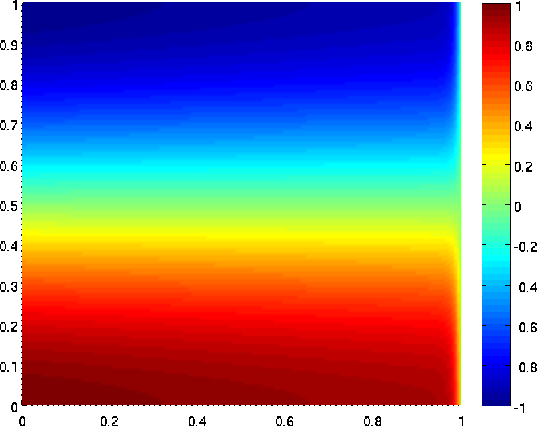
\includegraphics[scale=.24]{figs/wallBC_exact_u.png}
}
\subfigure{
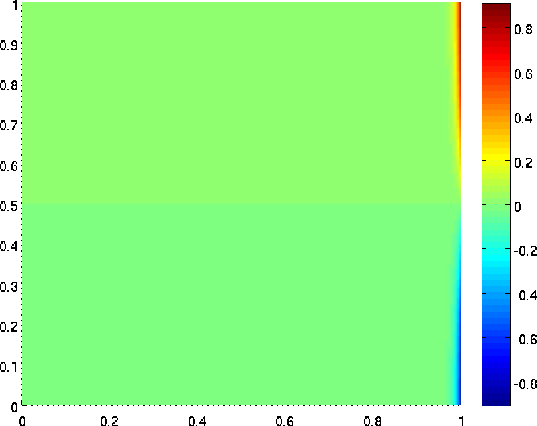
\includegraphics[scale=.24]{figs/wallBC_exact_sigx.png}
}
\subfigure{
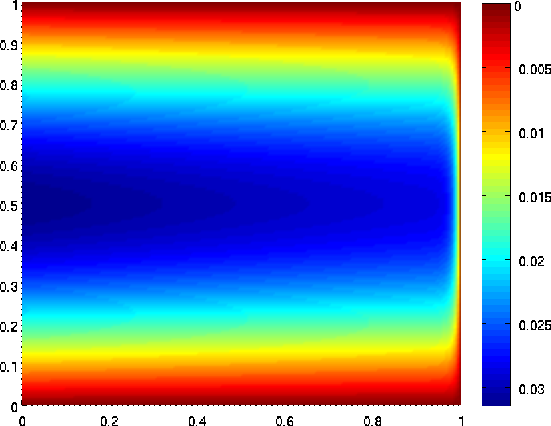
\includegraphics[scale=.24]{figs/wallBC_exact_sigy.png}
}
\caption{Solution for $u$, $\sigma_x$, and $\sigma_y$ for $\epsilon = .01$, $C_1 = 1$, $C_n=0$, $n\neq 1$}
\end{figure}
}

\frame{
\frametitle{Error rates}
\begin{figure}
\centering
\subfigure{
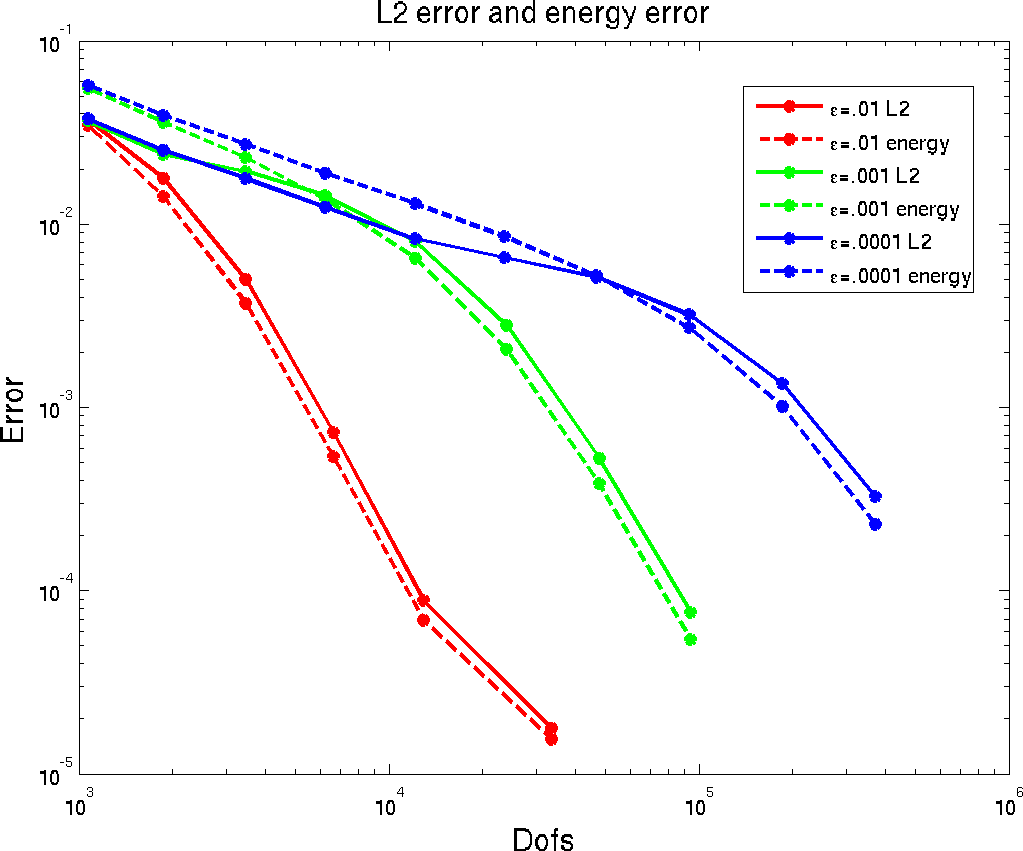
\includegraphics[scale=.23]{figs/errorrates_wallBC.png}
}
\subfigure{
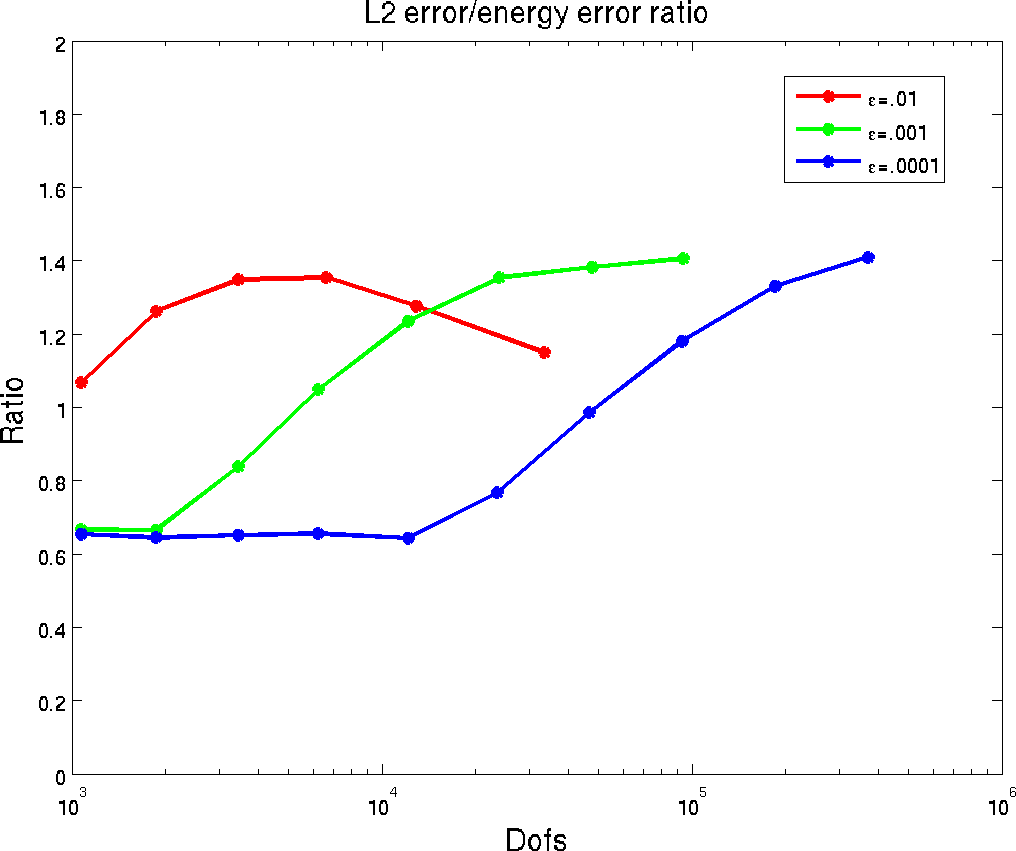
\includegraphics[scale=.23]{figs/L2energyratio_wallBC.png}
}
\subfigure{
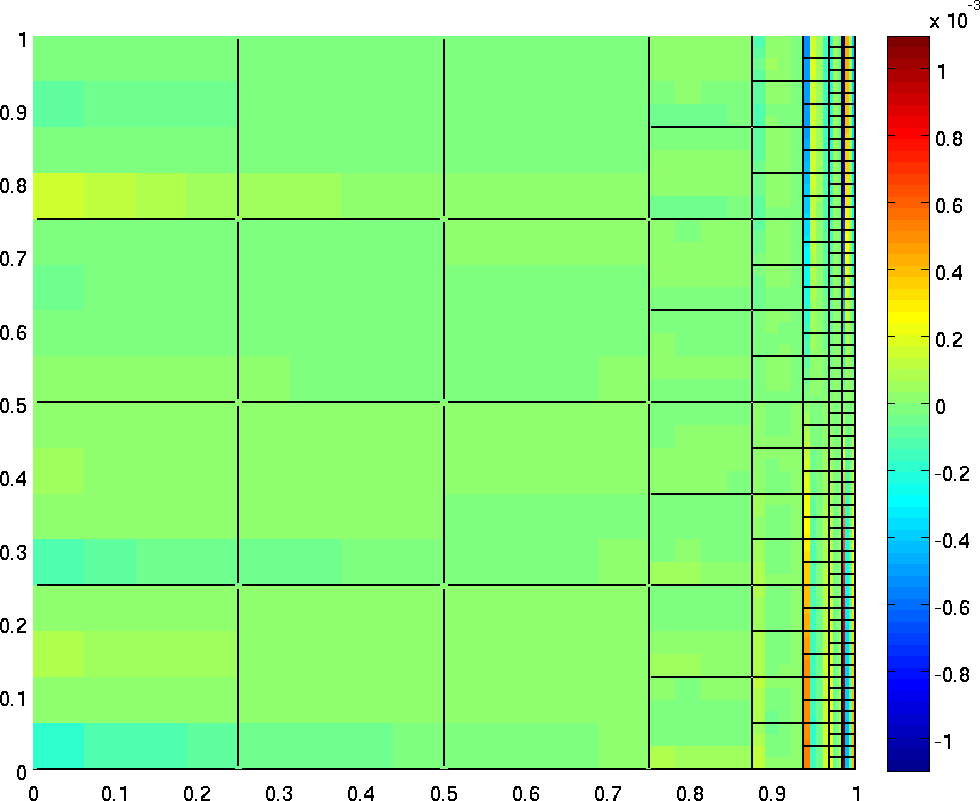
\includegraphics[scale=.22]{figs/u_pointdiff_wallBC.png}
}
\caption{$L^2$/energy error, their ratio, and pointwise error in $u$ for $\epsilon = .01$.}
\end{figure}
}

\frame{
\frametitle{Convection-diffusion as regularization}
Discontinuous inflow conditions on $\widehat{f_n}$, out of alignment with mesh. Boundary condition $\NVRgrad u \cdot n = 0$ at outflow.
\begin{figure}
\centering
\subfigure{
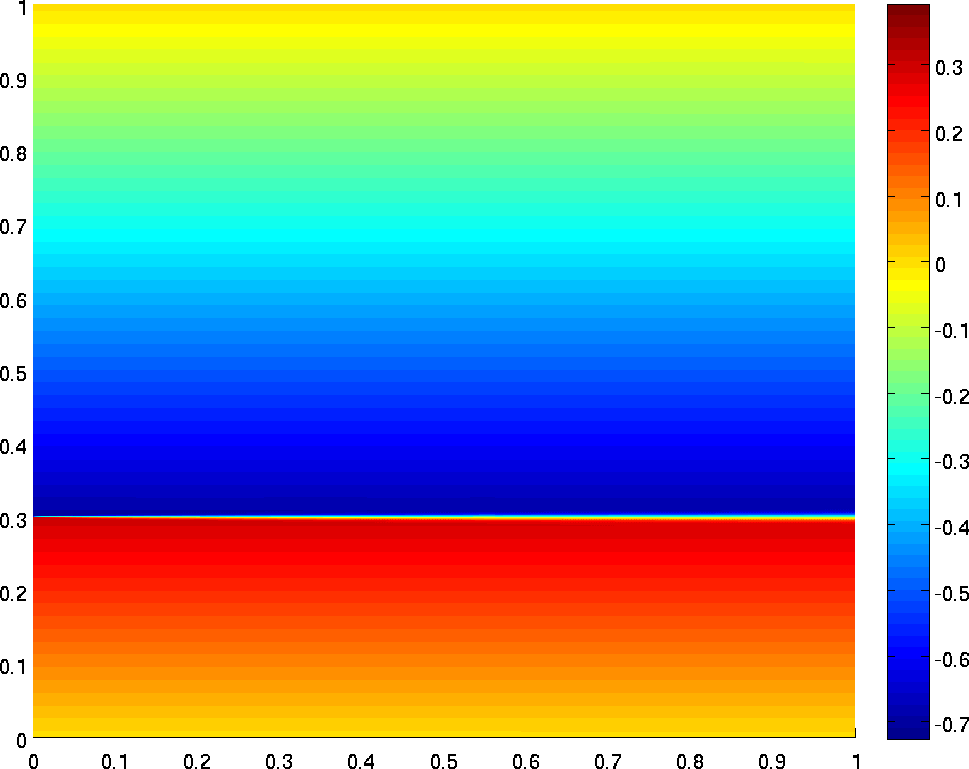
\includegraphics[scale=.33]{figs/discontinuous.png}
}
\subfigure{
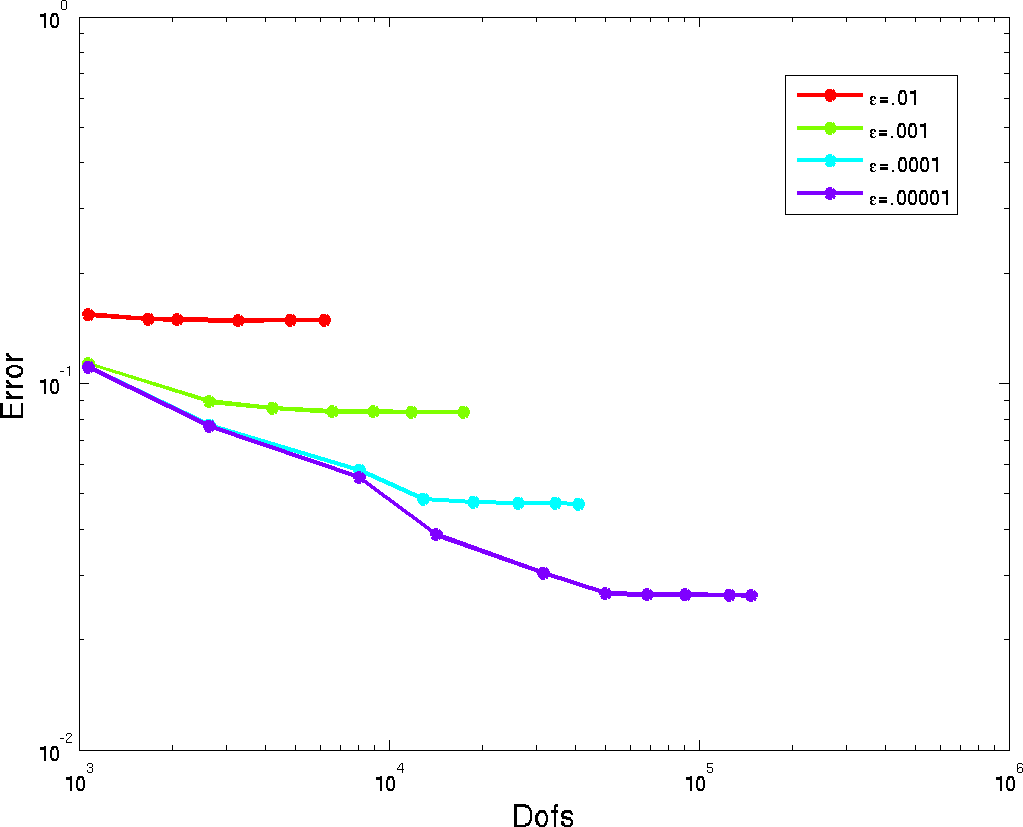
\includegraphics[scale=.305]{figs/discontinuousL2rates.png}
}
\caption{Discontinuous hat inflow data with $\epsilon = 1e-5$.}
\end{figure}
}

\frame{
\frametitle{Vortex problem}
For $\beta = (-y,x)^T$ on $\Omega = [-1,1]^2$, and zero normal stress outflow conditions. Ill posed in the convection setting.
\begin{figure}
\centering
\subfigure{

\includegraphics[scale=.33]{figs/vortex.png}
}
\subfigure{
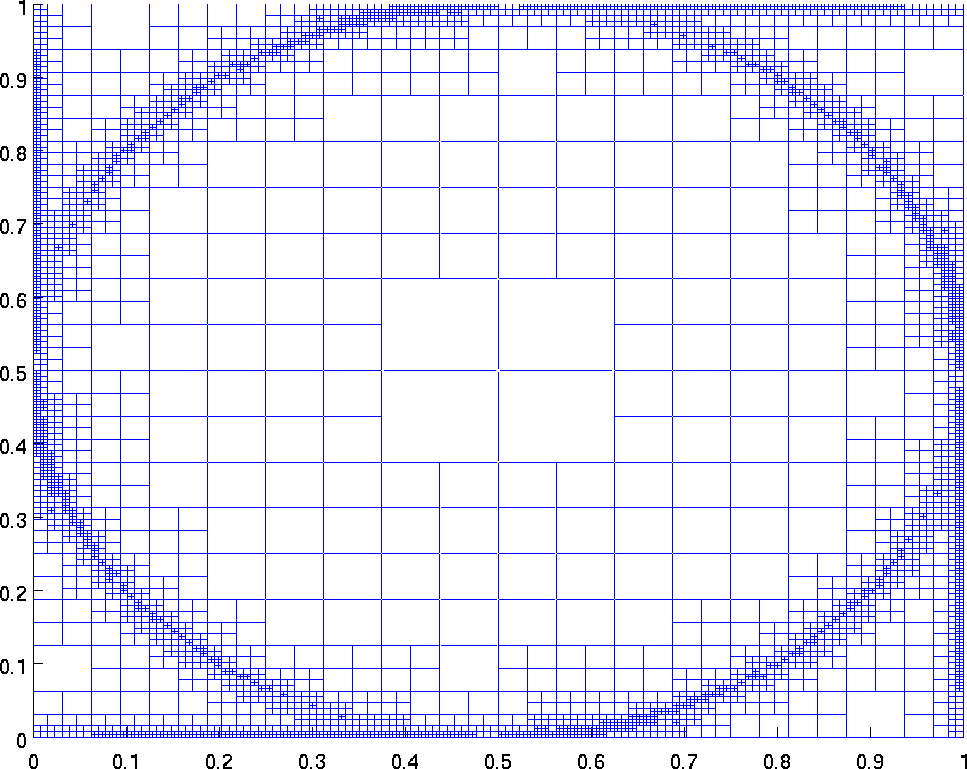
\includegraphics[scale=.33]{figs/vortexMesh.png}
}
\caption{Steady-state vortex problem with $\epsilon = 1e-5$.}
\end{figure}

}

\frame{
\frametitle{Burgers' equation}
\[
(u^2)_{,x} + (u)_{,y} - \epsilon \Delta u = 0
\]
with boundary conditions $u = 1-2x$ on $y\neq 1$, and $\NVRgrad u\cdot n = 0$ on $y=1$. 
\begin{figure}
\centering
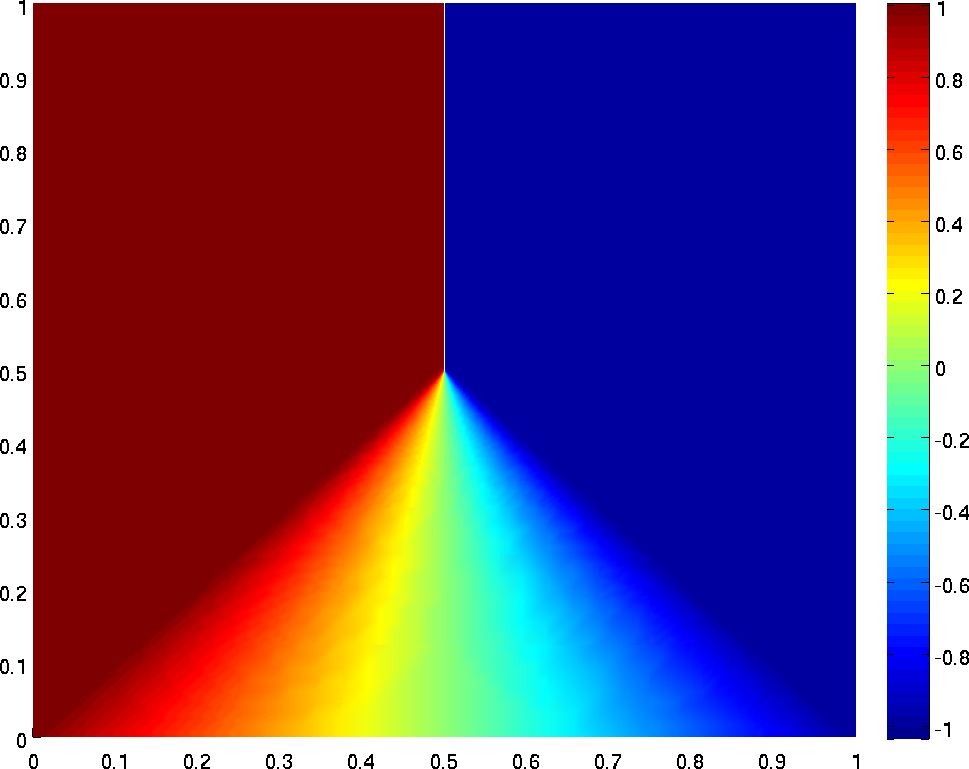
\includegraphics[scale=.35]{figs/burgers1e4.png}
\caption{Burgers' equation solution for $\epsilon = 1e-4$.}
\end{figure}
}


% --------------------------------------------------------------------------------------------------- 


\begin{frame}
\begin{thebibliography}{9}
\bibitem{robustness}
  Leszek Demkowicz and Jay Gopalakrishnan,
  \emph{A Class of discontinuous Petrov-Galerkin methods II: Optimal test functions},
  Numerical Methods for Partial Differential Equations,
  Volume 27, Issue 1, p70-105, January 2011

\bibitem{camellia}
  Nathan V. Roberts, Denis Ridzal, Pavel B. Bochev, Leszek D. Demkowicz,
  \emph{A Toolbox for a Class of Discontinuous Petrov-Galerkin Methods using Trilinos},
  Sandia Report SAND2011-6678,
  2011

\bibitem{robustness}
  Leszek Demkowicz, Norbert Heuer,
  \emph{Robust DPG method for convection-dominated diffusion problems}
  ICES Report 11-33,
  2011
  
\end{thebibliography}
\begin{center}
  \vfill
  Thank you.
  \vfill
  Questions?
  \vfill
\end{center}
\end{frame}

\end{document}
